\section{Konklusjon og anbefalinger}
\label{sec:konklusjon}
%\textit{Kort oppsummering av den innsikt som er oppnådd som er aktuelt for videreføring i Fase II. Enkelt-resultater som kan tallfestes bør være med.\\
%\\
%NB: Vær konkret på dette punktet. Det er uinteressant \textbf{at} gruppen har oppnådd innsikt på det ene eller andre området. Det interessante er \textbf{hvilken} innsikt som er oppnådd. %\\
%\\
%Anbefalinger for videreføring, bruk og vedlikehold er også viktig å få med.}


\subsection{Videreutvikling}

\subsubsection{Maskenettverk}

Systemet har slik det er nå en stor svakhet: aktivitet detekteres kun fra en side av turbinen, som kan gi store mørketall. Det vil også ikke oppdages om en fugl faktisk kolliderer med turbinen. Derfor vil det være lurt som en videreutvikling av systemet å utvide til en maskenettverk bestående av flere noder med hvert sitt kamera og prosesseringsenhet som vist i figur \ref{fig:maskenettverk}. Her har hver av nodene to-veis kommunikasjon med nabonoden og kan videresende data slik at alle noder kan kommunisere med hverandre. Dette gjør at node 1 og 3 fortsatt kan kommunisere med hverandre selv om node 2 feiler. En skisse av systemet i praksis rundt en vindturbin er vist i figur \ref{fig:fraoven}. Om en fugl detekteres på en side av turbinen, men ikke på den andre, vil et varsel kunne sendes til et menneske som kan undersøke om noe har kollidert med turbinen.

\begin{figure}[!htbp]
  \centering
  \begin{minipage}[b]{0.45\textwidth}
    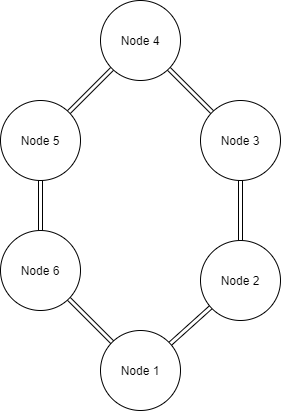
\includegraphics[width=\textwidth]{konklusjon/Mesh.png}
    \caption{Et tenkt maskenettverk for å dekke en hel vindturbin med seks noder. }
    \label{fig:maskenettverk}
  \end{minipage}
  \hfill
  \begin{minipage}[b]{0.45\textwidth}
    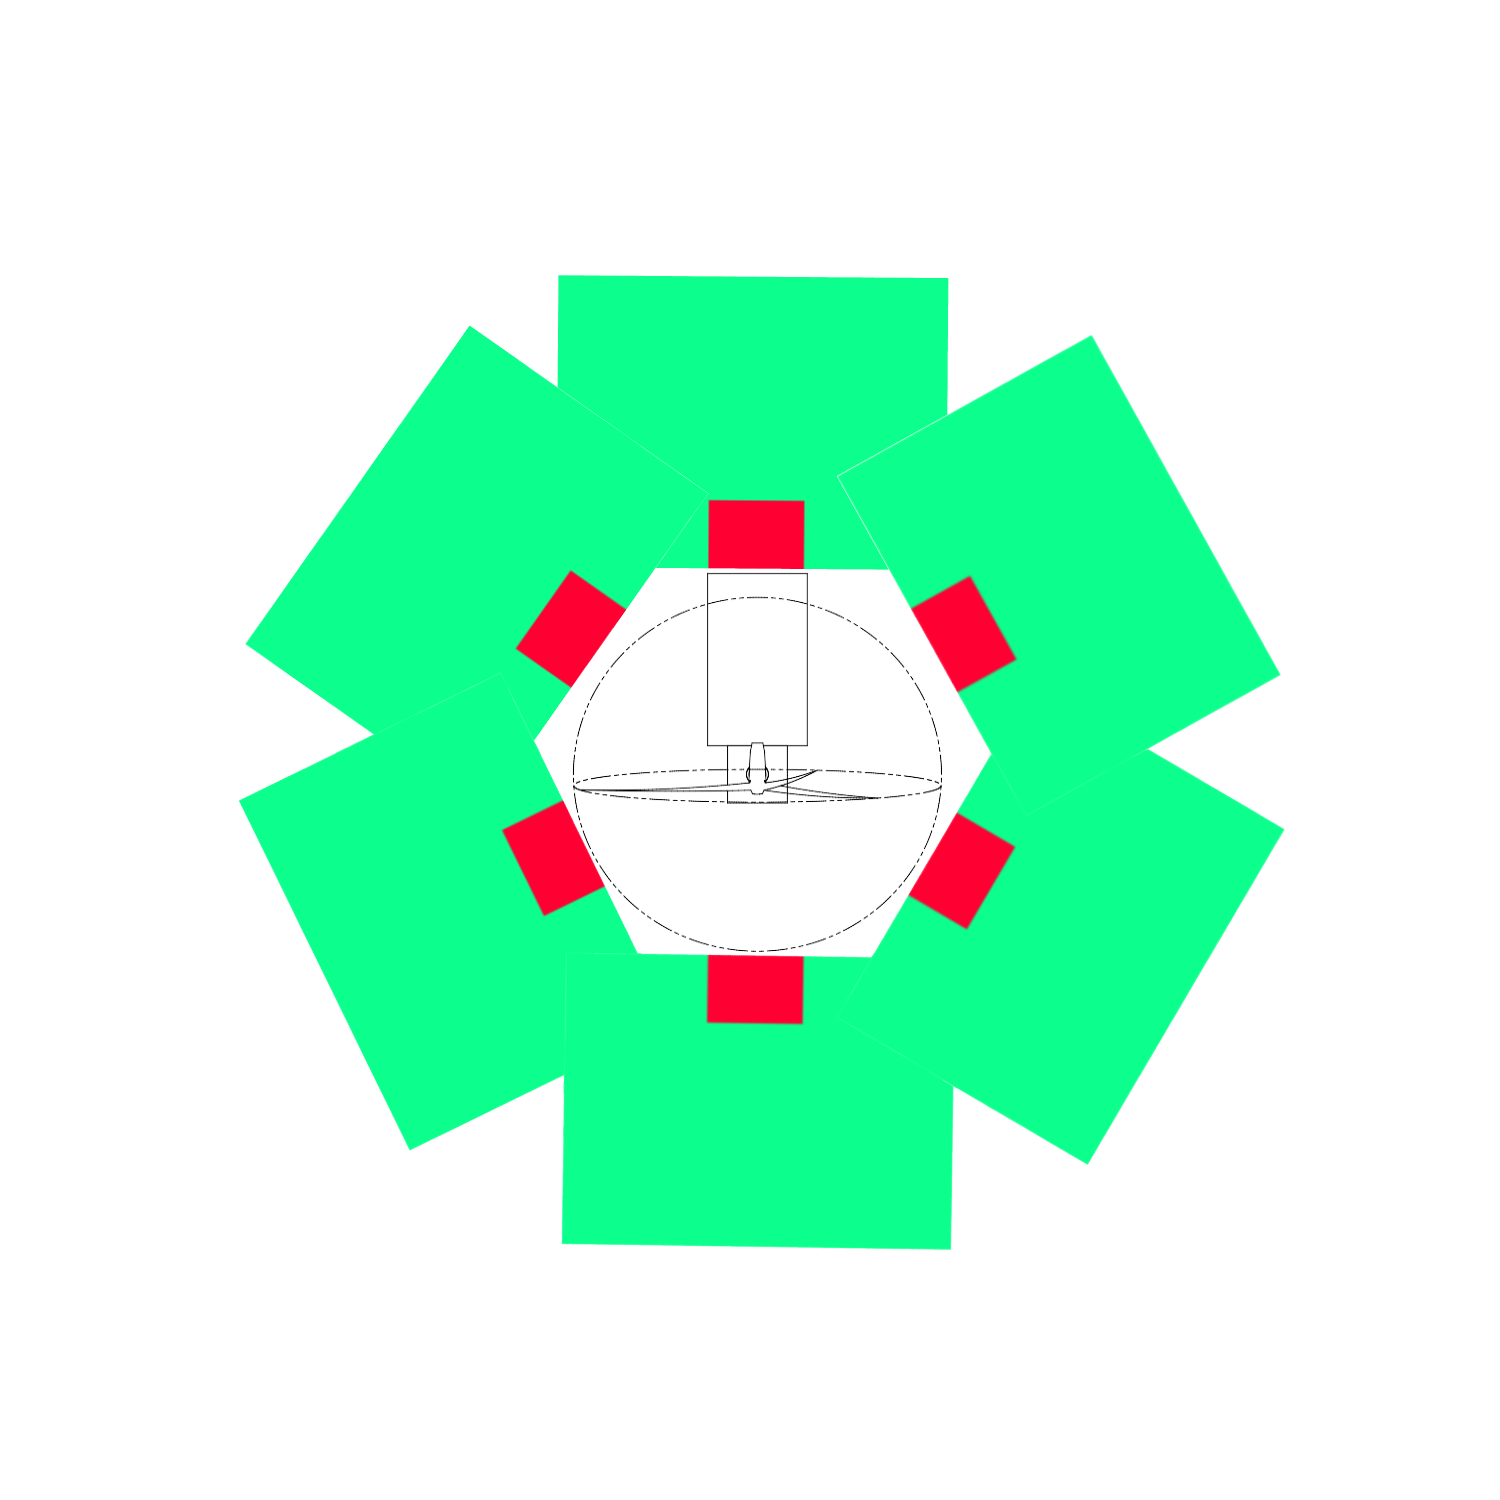
\includegraphics[width=\textwidth]{konklusjon/Nettverk.png}
    \caption{Konsept på hvordan seks kamera kan detektere fugletrafikk inn mot en vindturbin fra alle retninger. Det grønne området er deteksjonsområdet og rødt er boksenes plassering.}
    \label{fig:fraoven}
  \end{minipage}
\end{figure}





Dette kan også hjelpe i områder uten vindkraftutbygging der man skal telle fugler på et større område. Dette vil gi en høyere sikkerhet i antall talte fugler, der en fugl som ikke blir talt av et kamera kan bli telt av et annet. 

Det er to grunner til at dette ikke har blitt gjennomført: penger og tid. Kamera er den dyreste komponenten i systemet, der prisen for ett FLIR C3-kamera er på \$700. Det er også ansett som unødvendig å bruke tid på å utføre samme arbeid flere ganger i løpet av designprosessen til dette systemet.

\subsubsection{Synsvidde}
Om kameraet ikke ser nok foran vindturbinen vil det kunne være mulig å oppgradere kamera til et med større synsfelt. Dette vil gi hvert kamera et større område å detektere fugler på, og kan gi bedre data til å forutsi banen fuglen vil ta, da det vil være flere potensielle målinger.
%Om oppløsningen forblir den samme vil vi potensielt få færre piksler å jobbe med, som vil gi mindre nøyaktighet, men større område. Om oppløsningen blir skalert vil vi få lik nøyaktighet, men et større målingområde, som fører til større bilder i størrelse og da mer potensielt mer prosessering per bilde.

\subsubsection{Trådløshet}
For at produktet skal virke optimalt før vindturbiner er satt opp så vil dette kreve at systemet ikke bruker nettstrøm. Siden det prosesseres en bildestrøm kreves det mye prosessorkraft som igjen krever mye strøm. Store batterier er tunge, som senker mobiliteten til systemet, men vil kunne støtte mer prosessorkraft og også sørge for at systemet kan brukes over større tidsrom uten tilsyn.

%En pi4 på full load vil dra ca 1100mA. (\url{https://www.pidramble.com/wiki/benchmarks/power-consumption}). Om vi antar at kameraet drar full load på 600mAh\todo{ma, ikke mah} (ikke sikker)\todo{kilde} blir dette til 1700mAh. For at dette systemet skal fungere i over 24 timer krever dette et batteri med ca 41 Ah\todo{mah sier ingenting om energi. trenger wh}. Vårt mål er å detektere trender for fugleaktivitet over en lengere tid, som nå vil kreve et stort batteri om systemet skal over lengere tid. Dette er har ikke blitt gjort nå på grunn av tid, da vi ikke har tid til å optimalisere strømforbruket til systemet. 

\subsubsection{Ordinært bilde}

For enklere feilsøking og testing imens produktet står ute vil det være gunstig å supplementere IR-kameraet med et ordinært kamera som kan ta bilder når IR-kameraet detekterer en fugl. Dette vil kunne bli lastet opp til en database og bli observert av et menneske eller datamaskin, som kan bestemme art. Dette kan også brukes for å finne ut om systemet detekterer feil, altså om en detektert fugl var et falskt positivt resultat.

\subsubsection{Nettside og database}

Videreutvikling av nettsiden og databasen vil kunne være å legge til flere spesialiserte grafer for forskjellige data. Dersom det blir behov for et mesh-nettverk vil det også måtte være nødvendig å legge til funksjonalitet for å kunne støtte dette. Det kan være et kart der du kan se de forskjellige systemene og statistikk for hver enkelt node. 

Databasen har en svakhet, den er relativt treg, men veldig fleksibel. Det finnes flere løsninger som håndterer dette, men å gå over til en database som ikke er så fleksibel mot at den blir raskere er en mulighet. 


\subsection{Bruk}

Etter at systemet er satt ut i naturen skal det være autonomt, altså at det skal kunne detektere fugler og samle værdata samt laste opp data til databasen for analyse. Videre er det tenkt at om dataen som analyseres viser abnormiteter vil et menneske kunne dra ut til systemet og undersøke. Abnormiteter vil være kollisjoner, nedgang i aktivitet, og andre brudd på tydelige mønstre. Det er tenkt at dataen kan brukes av eierene av vindturbiner samt ornitologer for analyse. 

Vedlikehold vil tenkes å være omstart om systemet henger seg opp, fjerning av fremmedlegemer som blokkerer for linsen eller værstasjonen, samt å rette opp strukturen om den blir veltet av vind eller dyr. 

\subsection{Konklusjon}
Det designede, mobile systemet bruker et IR-kamera, en prosesseringsenhet og bildebehandling for å detektere, telle og spore fugler i kameraets synsfelt. Systemet sender antall fugler sammen med værdata fra egne sensorer til en database. En nettside henter data fra databasen og sorterer disse etter brukerens ønske. Treffraten på fugler er på 75\% i klart vær. Lavere treffrate når det er overskyet kommer i hovedsak av kalibrering diskutert i \autoref{sec:verifikasjon:kamera:kalibrering}. Samtlige systemkrav er tatt høyde for, men flere er ikke fullført.
\todo{må skrives mer her}
Vi kan konkludere med at alle undersystemene fungerer fra overvåking av fugleaktivitet og innsamling av værdata til presentering på en nettside, men systemet trenger å settes sammen før videre testing kan fullføres. Først da kan systemet være klart for å setteog forbedringer før det kan brukes autonomt\todo{riktig ord?}





\subsection{Takk}

Takk til institutt for elkraftteknikk for lån av FLIR C3. 

Takk til vår faglige veileder Bjørn B. Larsen.